\section{Results}
\label{sec:results}
% Numbers in this section come from PROGRESS.md, section 6 (P0 results), which is generated by
% scripts/p0_tables.py from the runs' rescore.json files. If a number changes there, change it here.
% All gains are signed so that positive means better, including LPIPS and DISTS (lower is better).

\subsection{P0: tier gain, filter gain and metric agreement}
\label{sec:results-p0}

\paragraph{Search.}
On \texttt{ugc\_strict}, every sampler improves the composite objective from 29.45 (naive upload)
to about 43--44 within 40 trials (\cref{tab:samplers}, \cref{fig:convergence}). Over five seeds,
GP-BO is the best and by far the most consistent sampler; TPE is second and random search third.
CMA-ES fails to reach the $\times2$ tier on two of five seeds within the budget: with a population
of 8, 40 trials are only five generations. The objective is reproducible, but the recipe is not:
all GP-BO seeds choose $\times2$ and a 4--6\,\% contrast increase, while grain (0--15) and the
unsharp amount (0.4--1.2) vary across seeds at the same score (43.77--43.80). The objective is flat
along these knobs.

\begin{table}[t]
  \centering
  \caption{Sampler comparison on \texttt{ugc\_strict} (composite, 40 trials, two training clips,
  five seeds). A sampler beats another if the difference of means exceeds both standard deviations.}
  \label{tab:samplers}
  \begin{tabular}{@{}lrr@{}}
    \toprule
    Sampler & Final best (mean $\pm$ sd) & Trial reaching 95\,\% of final gain \\
    \midrule
    GP-BO  & $\mathbf{43.79 \pm 0.02}$ & $17.4 \pm 8.0$ \\
    TPE    & $43.43 \pm 0.35$ & $16.2 \pm 5.5$ \\
    CMA-ES & $40.71 \pm 3.82$ & $22.4 \pm 6.6$ \\
    Random & $42.82 \pm 0.51$ & $15.6 \pm 10.3$ \\
    \bottomrule
  \end{tabular}
\end{table}

\begin{figure}[t]
  \centering
  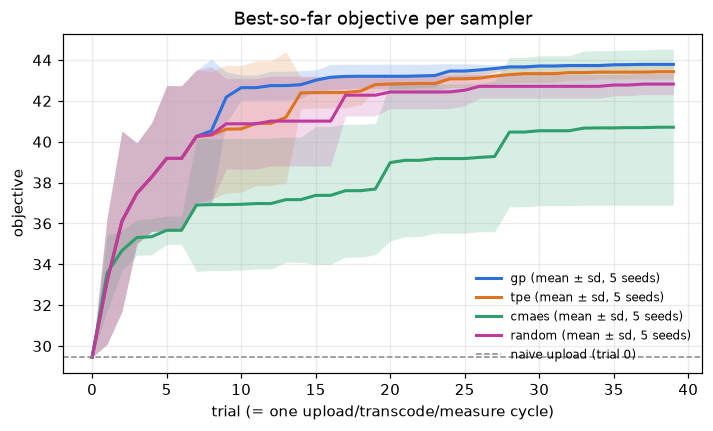
\includegraphics[width=0.75\linewidth]{p0/convergence.png}
  \caption{Best-so-far composite objective versus trial, mean and spread over five seeds per sampler
  (\texttt{ugc\_strict}).}
  \label{fig:convergence}
\end{figure}

\paragraph{Tier gain versus filter gain.}
\Cref{tab:e2} applies the decomposition of \cref{def:decomposition} and re-scores each configuration
with the judges. The tier gain ($\times2$ upload over naive) is confirmed by all three judges on all
four natural clips. The filter gain of the GP-BO configuration on \texttt{ugc\_strict} raises the
objective and both of its perceptual components on every natural clip, but it lowers SSIMULACRA2 and
XPSNR on every natural clip, and DISTS is flat. It is therefore not judge-confirmed. The same holds
for all five GP-BO seeds (0--1 of 3 judges). On \texttt{ugc\_av1} the filter gain passes the rule on
the means, but only because of one clip (park\_joy), where the AV1 tier-only upload is worse than the
naive upload on SSIMULACRA2 and the filters recover part of that loss.

\begin{table}[t]
  \centering
  \small
  \caption{Mean gain over the reference configuration on the four natural clips (park\_joy,
  old\_town\_cross, ducks\_take\_off, in\_to\_tree). The judges are SSIMULACRA2, DISTS and XPSNR;
  the last column counts judges with a positive mean gain.}
  \label{tab:e2}
  \setlength{\tabcolsep}{4pt}
  \resizebox{\linewidth}{!}{%
  \begin{tabular}{@{}lrrrrrrc@{}}
    \toprule
    Configuration (over reference) & composite & VMAF\textsubscript{NEG} & LPIPS & SSIMU2 & DISTS & XPSNR & judges \\
    \midrule
    Tier: $\times2$ over naive, \texttt{ugc\_strict} & +12.27 & +9.50 & +0.0657 & +23.02 & +0.0267 & +1.54 & 3/3 \\
    Filters: GP-BO over tier-only, \texttt{ugc\_strict} & +3.03 & +1.87 & +0.0280 & $-2.23$ & +0.0003 & $-0.75$ & 1/3 \\
    Filters: GP-BO over tier-only, \texttt{ugc\_av1} & +4.94 & +3.13 & +0.0437 & +1.90 & +0.0071 & +0.21 & 3/3$^\ast$ \\
    Learned $G$ (round 0) over tier-only & +2.55 & $-1.03$ & +0.0832 & $-5.17$ & +0.0101 & +1.24 & 2/3 \\
    \bottomrule
  \end{tabular}}\\[2pt]
  {\footnotesize $^\ast$Carried by park\_joy; on the other three natural clips SSIMULACRA2 and XPSNR are slightly lower.}
\end{table}

\paragraph{Where the filter gain comes from.}
Freezing contrast and saturation (\texttt{eq}) and re-running the search yields a sharpening-only
configuration ($\times2$, unsharp 0.89, $5\times5$, no grain). It keeps 72\,\% of the composite gain
and all of the LPIPS gain, and it passes two of three judges (DISTS $+0.0035$, XPSNR $+0.52$);
SSIMULACRA2 is still lower than tier-only ($-1.74$). The colour and contrast increase, together with
the grain that the optimiser adds alongside it, thus accounts for about 30\,\% of the composite gain
and turns XPSNR and DISTS negative. At the native tier ($\times1$, no tier change), a filter-only
search finds the same $+3.0$ composite gain almost entirely from an 11\,\% contrast increase, and no
judge agrees (0/3).

\paragraph{A Goodhart matrix.}
We optimise each of four objectives in turn and judge every result with all metrics
(\cref{fig:goodhart}). No objective is free of regressions on the metrics it does not optimise.
Optimising SSIMULACRA2 comes closest (one small regression, XPSNR $-0.24$) but gains little on its
own metric ($+0.54$). Optimising LPIPS alone saturates colour, sharpening and grain and is the worst
row on every other metric (SSIMULACRA2 $-14.9$).

\begin{figure}[t]
  \centering
  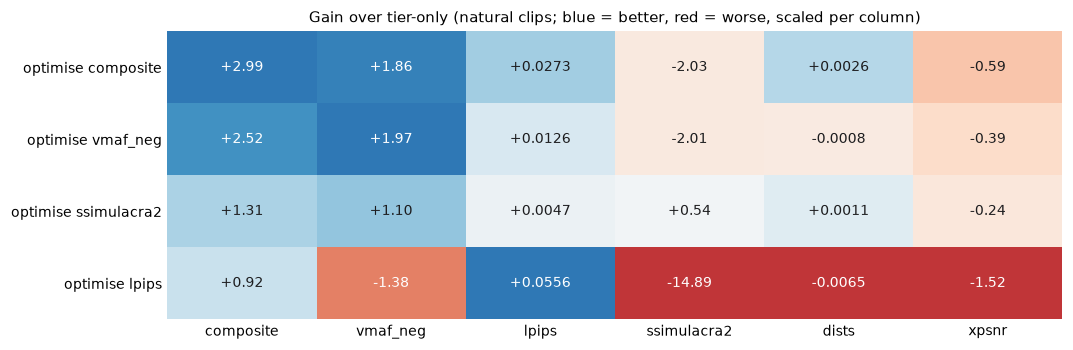
\includegraphics[width=0.8\linewidth]{p0/goodhart_matrix.png}
  \caption{Goodhart matrix. Rows: the objective optimised by GP-BO (40 trials). Columns: gain of the
  best configuration over tier-only, mean over the four natural clips, for each metric.}
  \label{fig:goodhart}
\end{figure}

\paragraph{Learned pre-compensation.}
Without a trust region ($\lambda=0$, $\delta=0.15$), the learned pre-compensation moves pixels by
18--32 levels on average; on its outputs the emulator's PSNR against the real playback falls to
19--25\,dB, and real quality collapses (old\_town\_cross: 60.4 for tier-only, 39.0 with $G$). With
the trust region, $G$ is above tier-only on the objective on three of four natural clips across
seeds (not on ducks\_take\_off), and, for seed 0, on XPSNR (4/4 clips) and DISTS (3/4); SSIMULACRA2
is lower on every clip in every seed (\cref{tab:e2}). Across seeds
(3 for $G$, 5 for the parametric configuration), $G$ beats the parametric configuration only on
old\_town\_cross and only on the objective ($65.39\pm0.87$ versus $62.62\pm0.16$); on the held-out
in\_to\_tree they tie, and the parametric configuration wins on SSIMULACRA2. $G$ damages the held-out
synthetic gradient clip far more than the parametric configuration ($-10.1$ composite over
tier-only). Domain-adaptation rounds did not improve the result.

\paragraph{Graphics and text.}
The parametric configuration found on natural clips lowers the composite of the synthetic test
pattern by 11.6 relative to tier-only, mostly through CAMBI's response to the added grain, and lowers
XPSNR by 7.0. Pre-compensation therefore has to be content-dependent, which motivates P1.

\subsection{P1: content-scoped learned pre-compensation}
\label{sec:results-p1}

\pending{E20: per-class baseline table (naive, tier-only, global sharpening-only, class-tuned
sharpening-only) on train and dev clips.}

\pending{E21: perceptual loss chosen for $G$ (LPIPS, DISTS or both) and the dev numbers behind the
choice.}

\pending{E22: global versus specialist $G$ on dev, 3 seeds; the pre-E23 decisions (the $G$ used for
class A, any additional nominated class, the gate table), with the commit in which they were frozen.}

\pending{E23: confirmation table for class A with bootstrap intervals; verdicts for H1, H2, H3; gated
system versus tier-only and the global sharpening-only configuration on all confirmation clips.}

\subsection{Real platforms}
\label{sec:results-p2}

\pending{P2 E15: measured ladder of one real platform (upload resolution and bitrate versus served
codec and bitrate), repeated uploads to measure non-determinism.}

\pending{P2 E16: real closed loop, naive versus tier-only versus sharpening-only versus the selected
configuration, with the number of uploads used.}

\pending{P2 E17: paired-comparison viewer study (tier-only versus sharpening-only versus $G$).}
